%TODO:

% - summary and discussion
% - literaturwert für kerr winkel


\documentclass[a4paper]{scrartcl}

\usepackage[utf8]{inputenc}
\usepackage[english]{babel}
\usepackage{lmodern}
\usepackage[T1]{fontenc}
\usepackage{booktabs}
\usepackage{multirow}
\usepackage{wrapfig}


% PAKETE
\usepackage{siunitx}
\usepackage{graphicx}
\usepackage{placeins}
\usepackage{longtable}
\usepackage{enumitem}
\usepackage{bbm}
\usepackage{sidecap}


\usepackage{amssymb} % math symbols
\usepackage{amsmath} % ams
\usepackage{amsfonts} % mathmatical fonts

% caption indenting
 \usepackage[format=plain,indention=0em,labelfont=bf,margin=1em]{caption}
 \usepackage{subfig} %subfigures ^^
\usepackage[protrusion=true,expansion=true]{microtype} % denser font, "-" behind line
\usepackage{esint} % nicer double and triple integrals
\usepackage{fancyhdr} % fancy headers
\usepackage[colorlinks=true,linkcolor=black,citecolor=black,filecolor=black,urlcolor=black]{hyperref}



% EINSTELLUNGEN
\sisetup{seperr,repeatunits=false}
\numberwithin{equation}{section}
\numberwithin{figure}{section}
\numberwithin{table}{section}

% EIGENE FUNKTIONEN
\newcommand{\re}{\operatorname{Re}}
\newcommand{\im}{\operatorname{Im}}
\newcommand{\gquote}[1]{\glqq #1 \grqq}

\newcommand{\eq}[2]{\begin{equation}#1\label{#2}\end{equation}}
\newcommand{\eqand}[0]{\hspace{.25cm} \bigwedge \hspace{.25cm}}
\newcommand{\grafik}[2]{\begin{figure}[h]\centering \includegraphics[width=10cm]{#1.eps} \caption{#2} \label{#1} \end{figure} }
\newcommand{\grafikq}[3]{\begin{figure}[h]\centering \includegraphics[width=10cm]{#1.eps} \caption[#2]{#3} \label{#1} \end{figure} }
\newcommand{\tbl}[3]{\begin{table}[h]\caption{#1}\label{#2}\begin{center}#3\end{center}\end{table}}
\newcommand{\Abbildung}[1]{\textsl{Abbildung \ref{#1}}}
\newcommand{\AbbildungI}[1]{\textsl{(Abbildung \ref{#1})}}
\newcommand{\Tabelle}[1]{\textsl{Tabelle \ref{#1}}}
\newcommand{\TabelleI}[1]{\textsl{(Tabelle \ref{#1})}}
\newcommand{\Formel}[1]{(\ref{#1})}
\renewcommand{\d}{\mathrm{d}}
\newcommand{\ve}[1]{\mathbf{ #1} }

\title{Ma 12: Magneto-optic Kerr effect and Magnetic Anisotropy}
\subtitle{Tutor: B. Lewitz}
\author{Benjamin Huber, Carolin Wille}
\date{November 21, 2011}

\begin{document}
\thispagestyle{empty}
\maketitle
\tableofcontents
\clearpage


\section{Introduction}
The magneto-optic Kerr effect (MOKE) describes the changes in the polarization of light, which is reflected from the surface of a magnetic material. Therefore it can be used to analyse magnetic properties, such as the structure of magnetic domains or the phenomenon of hysteresis effects. It has a great application in magneto-optic data storage like in magneto-optic discs, which are written magnetically and read out optically making use of the Kerr effect. The Kerr effect is also used in Kerr microscopes, which directly show the structure of magnetic domains.

\subsection{Magneto-optic Kerr effect}
The magneto-optic Kerr effect is a quantum mechanical scattering effect. However, it can be qualitatively understood in the picture of classical electrodynamics. Therefore, we consider a light-wave, that is reflected from a surface. During the reflection process it
 penetrates into the material, before it is emitted again. During the time, the wave spends in the solid, the dielectric displacement $\ve D $ has to be considered instead of the electric field $\ve E$. The quantities are related via
\eq{\ve D_i = \epsilon_{ij} E_j \;, } {DE}
where $ \epsilon_{ij}$ is the permittivity tensor, that reduces to a scalar for isotropic materials. In magnetized materials, the tensor $\epsilon_{ij}$ decomposes into a real isotropic ($\alpha_{ij}$) and an imaginary totally antisymmetric ($\beta_{ij}$) contribution
\eq{\epsilon_{ij} = \epsilon_0 \alpha_{ij} + i \beta_{ij} \; . }{eps}
As the antisymmetric tensor $\beta_{ij}$ has vanishing diagonal entries, it can be expressed in terms of a cross-product with the so called gyration vector, that can be identified in a classical picture with the direction of the magnetic field $\ve j$. Equation \Formel{DE} can then be written as
\eq{\ve D = \epsilon_0 \ve E - i \epsilon_0 Q \ve j \times \ve E \; , }{DEJ}
where $\epsilon_0$ is the vacuum permittivity and $Q$ is a complex material constant, that is approximately proportional to the magnetization. The cross-product in equation \Formel{DEJ} describes a rotation around the magnetization axes by $\pi/2$, that can be described as a Lorentz force, which is acting on the electrons, that are oscillating in the material due to the periodic excitation of the incoming wave. However, the magnetic field, which would cause a Lorentz force needed to describe the rotation deviates significantly in orders of magnitude when compared to the real magnetic field. Therefore this classical picture has to be used with caution.

A further analysis of the Maxwell equation for this problem \cite{dissert} leads to the conclusion of different refraction indices and amplitudes for left and right circular polarized light. As linear polarized light is nothing but a superposition of these two, it becomes clear, that its direction is rotated as a result of the phase shift between the two components and is furthermore polarized elliptically due to the different intensities (cf. fig. \ref{fig:kerr}).



\begin{figure} 
 \centering
\subfloat[][Kerr and Faraday Effect]
{         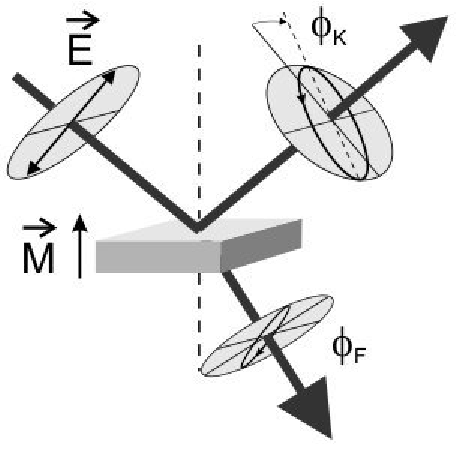
\includegraphics[width=0.4\linewidth]{img/kerrpic.pdf}
       
}
% \hfill
\subfloat[][Types of MOKE]
         {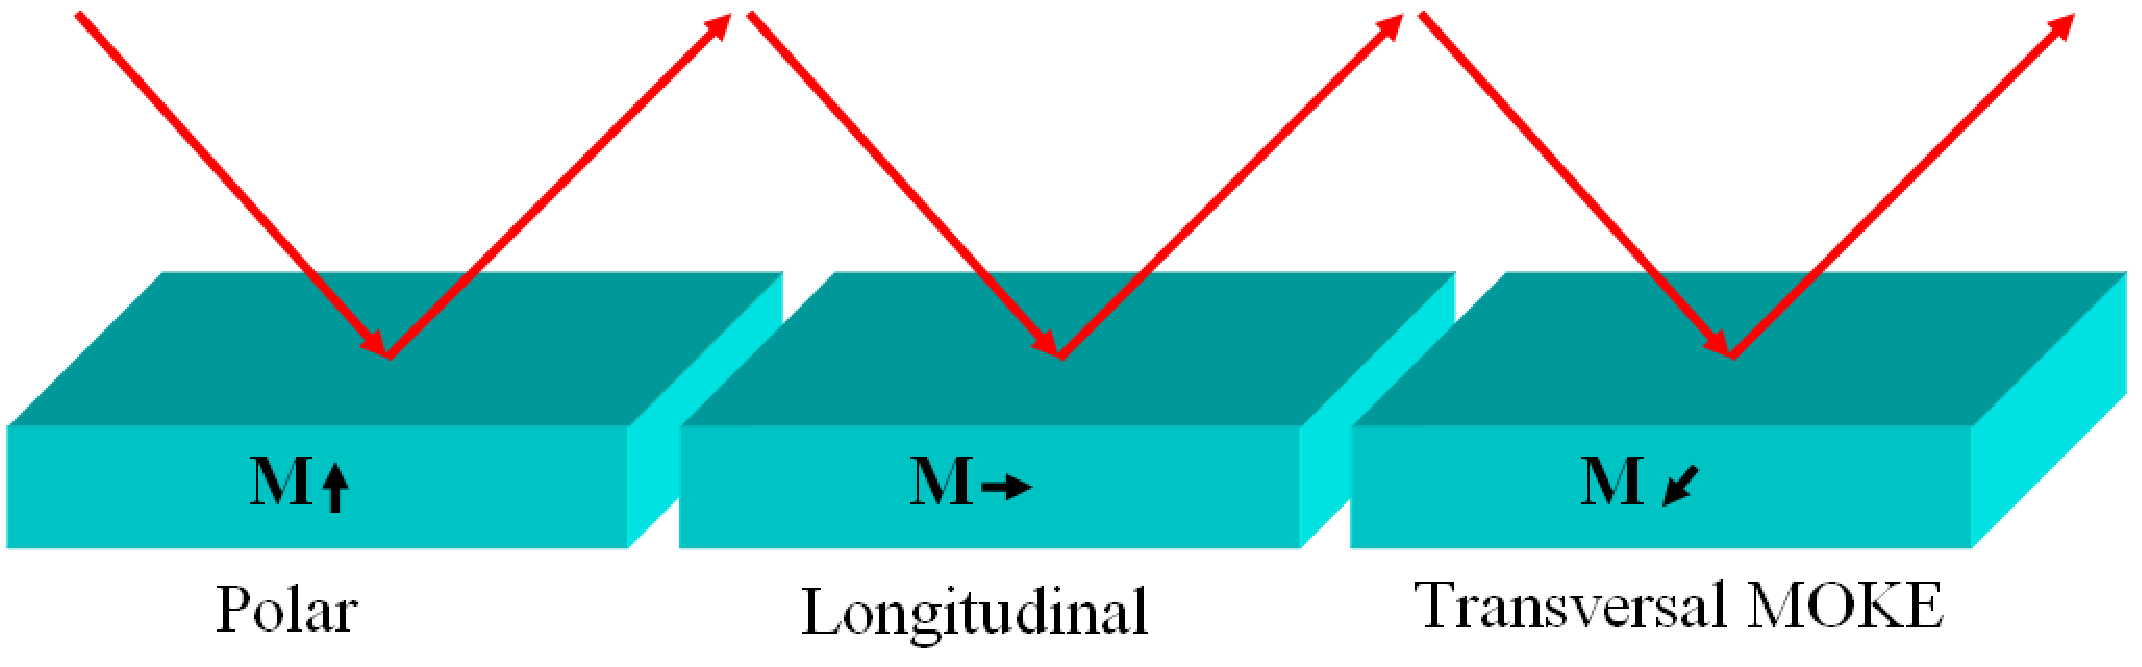
\includegraphics[width=0.6\linewidth]{img/moke.pdf}}

\caption{
\small $\ve a)$ Schematic description of the Kerr effect (polar) characterized by the Kerr angle $\phi_K$. The same effect occurring for the transmission of light is called Farrady effect \cite{dissert}. $\ve b)$ According to the direction of the magnetization of the sample $\ve M$ and the incidence plane three different types of MOKEs are characterized. 
Source: \url{http://en.wikipedia.org/wiki/Magneto-optic_Kerr_effect}. } 
	\label{fig:kerr}
\end{figure}




\subsection{Magnetism}
Magnetic dipoles exert a force on each other, causing the configuration of dipole orientation with minimal energy to be the one with all dipoles pointing in the same direction. This causes two important magnetic effects.

\subsubsection*{Magnetic Domains}
On a small scale all dipoles tend to point in the same direction. Globally though, a large extended magnetic field is energetically sub optimal. Instead, different regions, so called domains emerge with parallel dipoles within the domain, but different orientations between regions. The domain walls consist of small regions where the dipoles change gradually from one to the other orientation by rotating either around an axis parallel (N\'{e}el wall) or perpendicular (Bloch wall) to the wall.

This construct can globally be neutral, resulting in no significant macroscopic field, but will generally prefer the direction of an external magnetic field. With increasing external field strength more and more domains change orientation until all magnetic dipoles are parallel (cf. figure \ref{fig:doms}).
\begin{figure}
        \begin{center}
         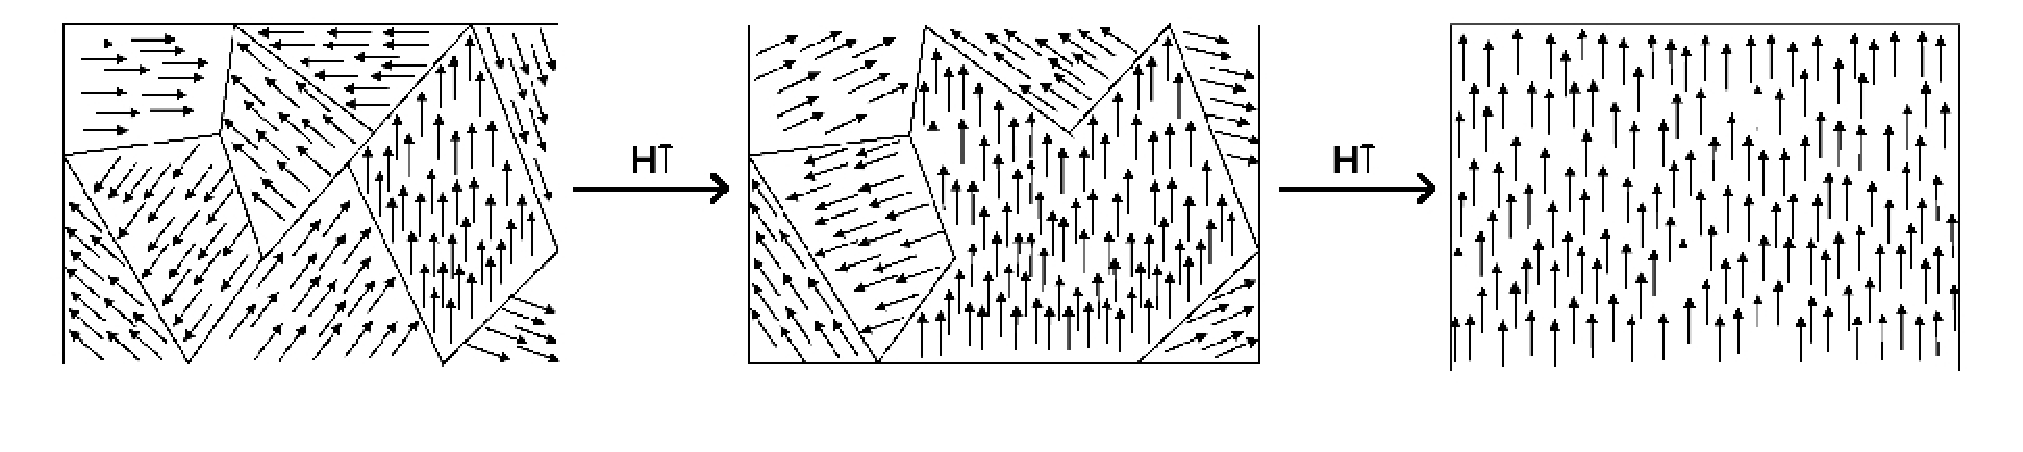
\includegraphics[width=0.9\linewidth]{img/Dominios.pdf}
        \end{center}
        \caption{
\small Rotation of orientation and increase in size of magnetic domains due to an externally applied field. Picture taken from \url{http://en.wikipedia.org/wiki/Magnetic_domain}.
        }
        \label{fig:doms}
\end{figure}

\subsubsection*{Magnetic Hysteresis}
Decreasing the external field after all domains were parallely oriented reverses the above effect and creates or enlarges domains with different orientation little by little. As the orientation flipping requires energy though, it will only happen, if the difference in total energy between the current and the flipped state is larger than this required energy. Thus there will be more domains with the original orientation, even after the external field has vanished. This remaining macroscopic magnetic moment is called the remanence magnetisation. An opposing field with the so called coercivity strength is required to completely demagnetize the material. The different magnetizations while increasing and decreasing the external field create the so called hysteresis curve (cf. figure \ref{fig:hys}).
\begin{figure}
        \begin{center}
         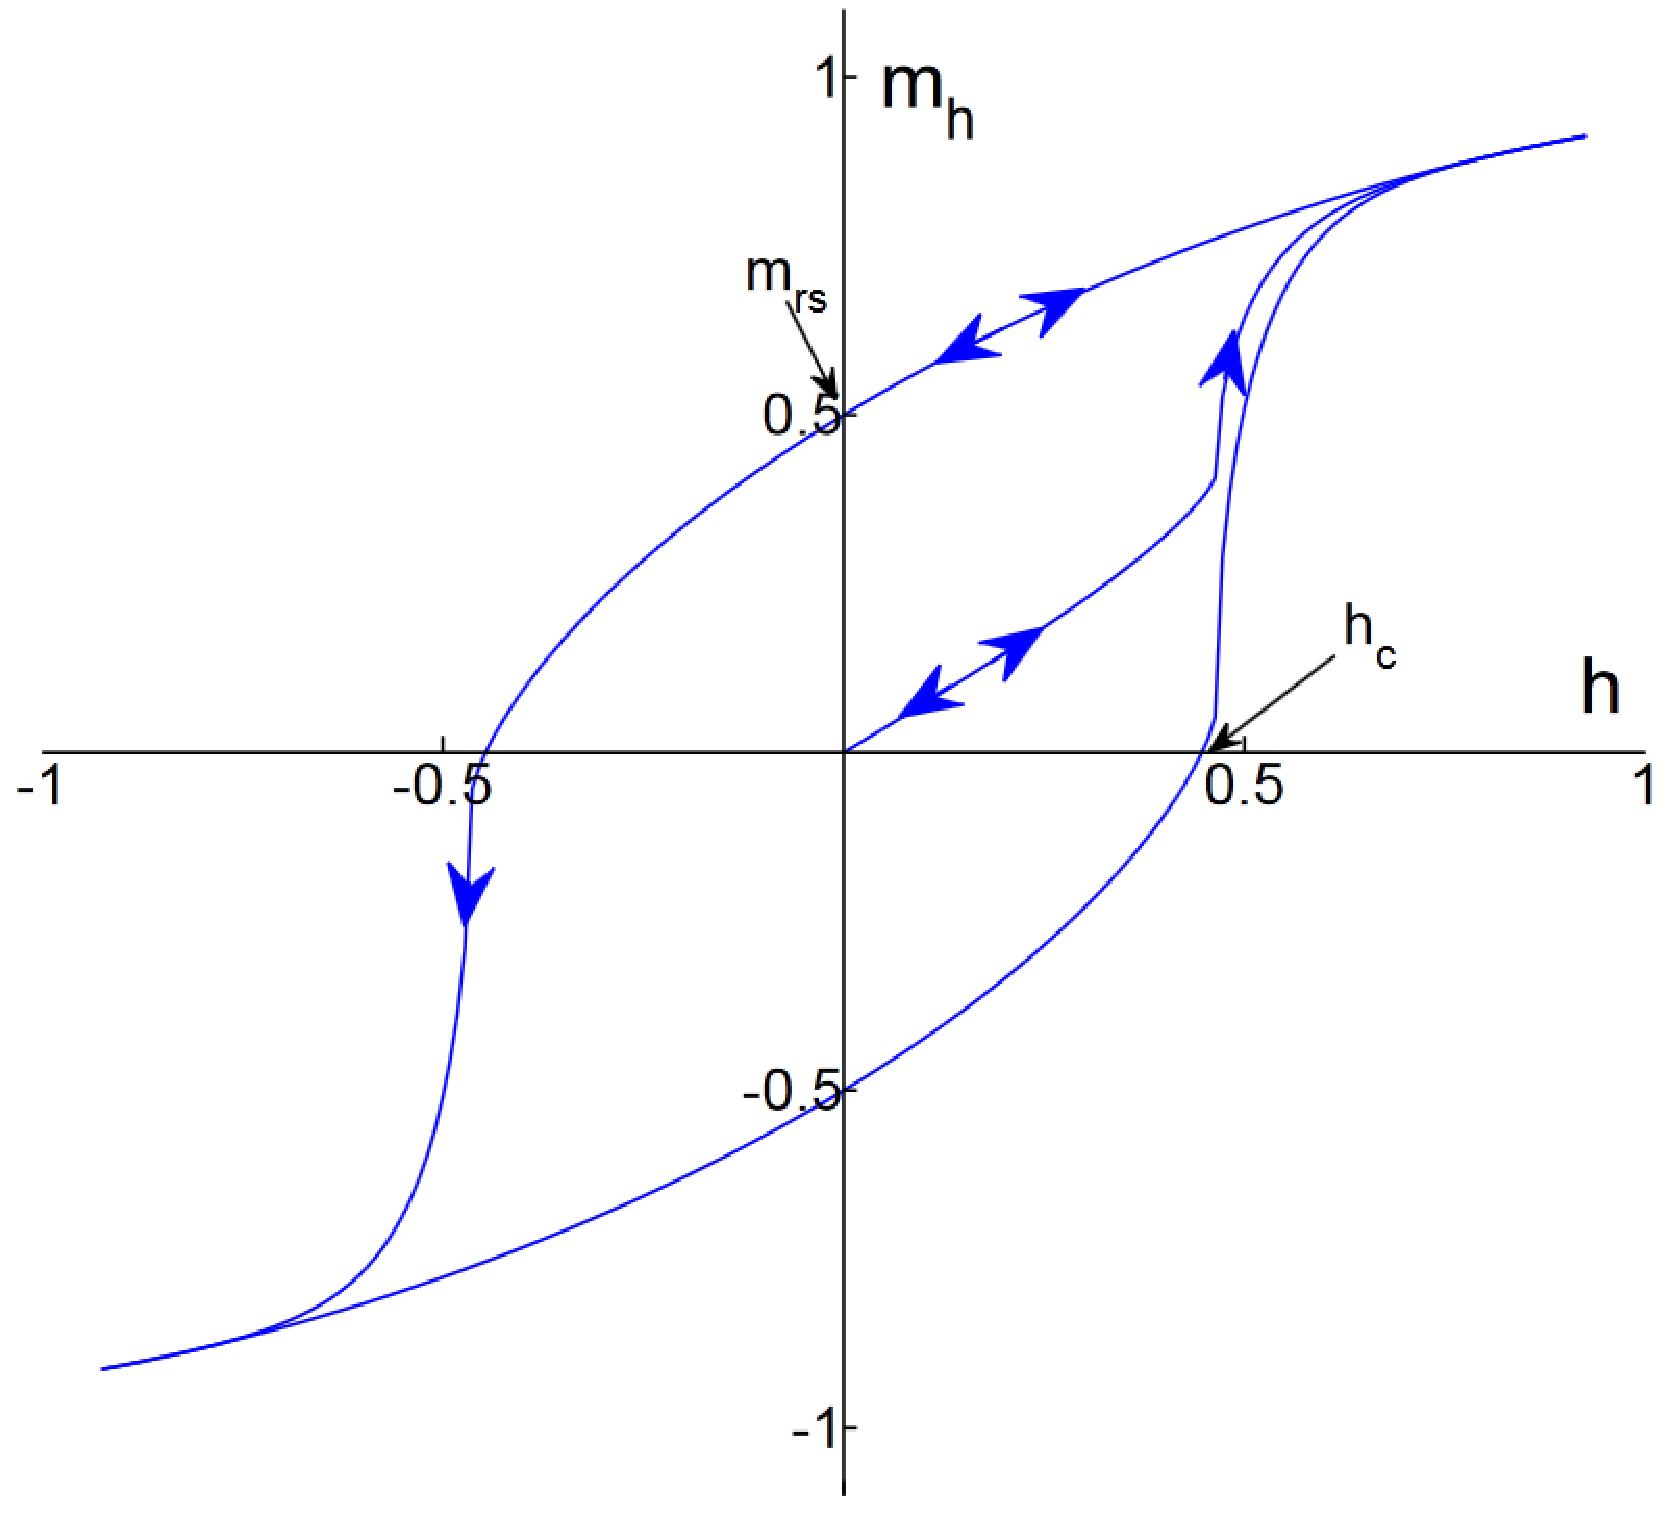
\includegraphics[width=0.31\linewidth]{img/hys.pdf}
        \end{center}
        \caption{
\small A plot of magnetization $m$ against magnetic field $h$ calculated using a theoretical model. Starting at the origin, the upward curve is the initial magnetization curve. The downward curve after saturation, along with the lower return curve, form the main loop. The intercepts $h_c$ and $m_{rs}$ are the coercivity and saturation remanence. Picture taken from \url{http://en.wikipedia.org/wiki/Hysteresis}.
        }
        \label{fig:hys}
\end{figure}


\subsubsection*{Magnetic Anisotropies}
A ferromagnet usually energetically prefers a certain direction of magnetization. This effect is called magnetic anisotropy and results mainly from two different contributions.

The shape of the magnetic sample is important as the stray field caused by the long range dipole-dipole interaction is dominated by the geometry of the sample. For thin films, the favorable magnetization direction lies within the plane of the film.

The other contribution is called the crystal anisotropy. It is a result of the spin-orbit interaction in every atom of the lattice and describes the fact that the magnetization direction along the different crystal axes result in different energy contributions. The crystal axes, which lead to minimal energy contribution are called "easy axes" in contrast to unfavorable axes, that are called "hard axes". For a small deviation of the angle $\Theta$ between the magnetization direction and the direction of the easy axis, the crystal anisotropy energy is given by
\eq{E_c=K \cos^2 \Theta \sin^2 \Theta \; , }{eq:aniso}
where $K$ is the anisotropy constant in this lowest order approximation.


%\section{Experimental Set-Up}
%oder machen wir noch mehr zum aufbau? sonst brauchen wir das kapitel nicht so zu nennen...
\subsection{Determination of Kerr Angle}
The rotation angle of the Kerr rotation is $\Phi_K$ and can be analyzed using a polarization filter, that is also called analyzer. While it is not possible to measure the rotation directly, the evolution of the intensity depending on the angle $\alpha$ is known to be
\eq{I(\alpha)=I_0 \cos^2(\alpha-\alpha_0) ,}{eq:malus}
where $\alpha_0$ is the angle of polarization. This equation as stated only holds for linearly polarized light, but in general circular or elliptically polarized light can be described as a superposition of two perpendicularly polarized light beams. The law thus becomes
\eq{I(\alpha) = I_0 \cos^2(\alpha-\alpha_0) + I_1 \sin^2(\alpha-\alpha_0) .}{}

It can be convenient to look at another value, that is useful to have at any rate: the contrast $c$. It is defined as the difference between minimum and maximum value devided by the offset (their average). In our case these minima and maxima are simply the intensities at the opposing saturation magnetisations.
\eq{c(\alpha)=\frac{\Delta I(\alpha)}{<I(\alpha)>} = 2\frac{I_+(\alpha)-I_-(\alpha)}{I_+(\alpha)+I_-(\alpha)} \; .}{eq:contrast}
Where the two saturation intensities can be calculated by the above equation \Formel{eq:malus}
\eq{I_\pm(\alpha) = I_0 \cos^2(\alpha-\alpha_0\pm\Phi_K) + I_1 \sin^2(\alpha-\alpha_0\pm\Phi_K) \; ,}{}
where $\alpha_0$ now is the angle of the incident light. Combining this with \Formel{eq:contrast} results in
\eq{c(\alpha) = \frac{2(I_1-I_0) \sin(2(\alpha-\alpha_0)) \sin(2\Phi_K) } { I_0+I_1+ (I_0-I_1)\cos(2(\alpha-\alpha_0)) \cos(2\Phi_K)} .}{eq:c}



\subsection{Theoretical Calculation of Magnetic Field}
By the use of Ampere's Law, we obtain for a toroid coil with an iron core, that has radius $r$, winding number $n=300$ and a slit of width $d=\SI{12}{mm}$
\eq{nI=\oint_{\mathcal S} \vec{H} \cdot \mathrm{d}\vec{s} = 2 \pi r H_{Fe} + d H_{Air} \;, }{Htheo}
where $I$ is the current that runs through the coil. As the relative permeability for iron is by approximately a factor $3000$ higher then the permeability of air and the radius of the coil is not by orders of magnitudes larger than the slit width, we can neglect the first summand in \Formel{Htheo} yielding
\eq{B_{slit} =  \mu_0  H_{Air}= \frac{\mu_0 n}{d} I = \SI{31.4}{mT A^{-1}} I \; .}{}

\FloatBarrier
 
\section{Analysis}
\subsection{Calibration}
\label{sec:cali}
While it is easily possible to calculate the maximum magnetic field from the winding number and core material, it is rather difficult to account for all details like displacement from the center, magnetic remanence in the core and so on. To get an accurate value of the magnetic field in our setup nonetheless, an initial measurement with a Hall probe was performed at the future position of the sample. Figure \ref{fig:cali} shows the correlation between coil current and measured voltage for both, the center of the coil and the sample position. Furthermore the hysteresis of the iron core is clearly visible. To account for this offset, all following curves will be considered not against the coil current, but the corresponding magnetic field resulting from the current branch of this hysteresis curve.

To have an easy functional relation, a linear function was fitted to a linear part of every branch. The endpoints will not be correctly represented, but will not be used for any calculations either way. The error of these fits is negligible compared to other sources of inaccuracy in future measurements.
\begin{figure} 
 \centering
\subfloat[][center]
{         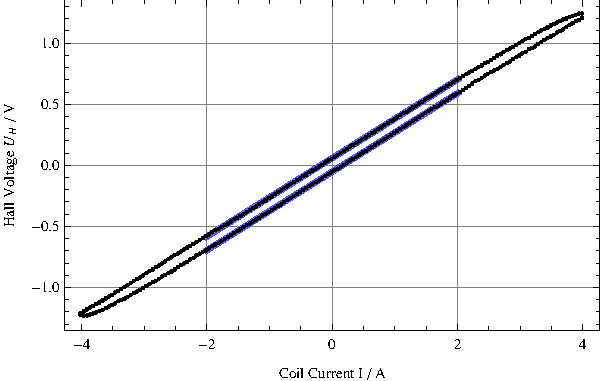
\includegraphics[width=0.45\linewidth]{img/calicenter.pdf}
       
}
\subfloat[][sample position]
         {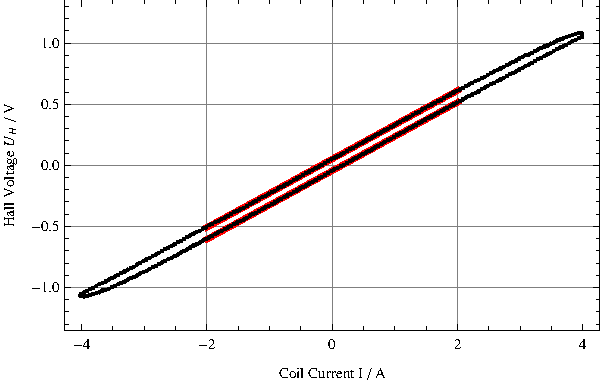
\includegraphics[width=0.45\linewidth]{img/calisample.pdf}}

\caption{
\small Hall voltage against the coil current for the center of the coil \textbf{(a)} and the position of the sample \textbf{(b)}. For future use, linear functions are fitted with all measured points between $I=-2\,\text{A}$ and $I=+2\,\text{A}$ (fits plotted for emphasis). } 
	\label{fig:cali}
\end{figure}


\subsection{Magnetic Anisotropy}
Due to difficulties to perform this in the setup, not small deviations (as described e.g. in formula \ref{eq:aniso}) but the full [100] and [110] directions were measured. According to \cite{kittel} the following term is expected as the anisotropy energy density:
\eq{U_K=K_1(\alpha_1^2\alpha_2^2 + \alpha_2^2\alpha_3^2 + \alpha_1^2\alpha_3^2) + K_2\alpha_1^2\alpha_2^2\alpha_3^2 .}{}
Due to this term vanishing for the [100] direction, this direction requires less energy to be magnetized. The [110] direction on the other hand has an additional term of $K_1 / 4$ compared to the easy direction. In the hysteresis curves this difference is notable (cf. figure \ref{fig:ani}). It is expected, that the area between the two plots (being an energy density) corresponds to this additional term.

After aligning the to curves by finding the best overlay of the end (saturated and linear) parts and recalibrating them to be at $2.1\,$T (cf. \cite{skript}), the two linear fits (cf. figure \ref{fig:ani}) result in an area and thus anisotropy constant of
\eq{K_1 = (44.0\pm 5.3)\frac{\text{kJ}}{\text{m}^3},}{} 
where the error is solely due to the noise in the curve / fit. This value is identical to the literature value of $K_1=42\frac{\text{kJ}}{\text{m}^3}$ from \cite{kittel}. The upper part of the curves could not be evaluated due to an unknown deformation in the hard hysteresis curve.
 
\begin{figure} 
 \centering
\subfloat[][full hysteresis curve]
{         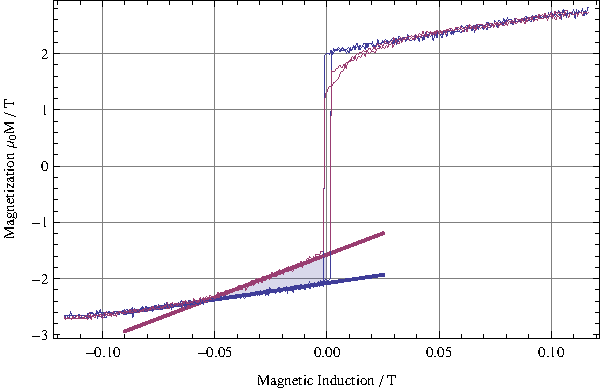
\includegraphics[width=0.45\linewidth]{img/ani.pdf}
       
}
\subfloat[][enlargement]
         {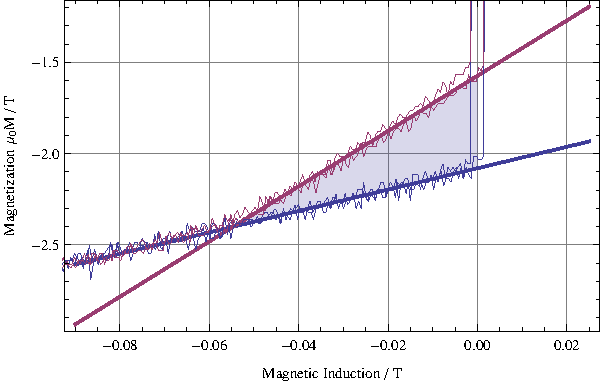
\includegraphics[width=0.45\linewidth]{img/anilarge.pdf}}

\caption{
\small Hysteresis curves of an easy ([100], blue) and harder ([110], purple) axis. Magnetization $\mu_0 M$ in Tesla (calibration via the relation $\mu_0 M = 2.1\,\text{T}$) against magnetic induction in Tesla from the calibration in section \ref{sec:cali}. Area (shaded) between the two curves is estimated by two linear functions fitted to the linear parts between -0.05 and -0.005. } 
	\label{fig:ani}
\end{figure}


\subsection{Drift}
During the measurements, there was a (periodic?) drift notable from time to time that resulted in a set of curves that had to be redone. The zero measurement, that was done to try and get a quantitative hold on this phenomenon, showed a large variation in recorded intensity. As there was no coil current in these measurements, the full course of these curves can be seen as unwanted noise (see. fig \ref{fig:waal}). There is a whole list of possible causes. Apart from defect instruments and heating of sample and photodiode a mechanical reason appears to be the most probable. The short lived spikes seen in the top-most curve in fig \ref{fig:waal} correspond to a door being closed. Thus an influence from mechanic disturbances or resonances are obviously possible.

Irrespective of the unknown cause for these drifts in measured intensity, they can not be ignored for the error considerations. While a quick change in intensity will result in a skew (not closed) hysteresis curve and thus be ignored for the calculations (as only measurements with well defined hysteresis loops were evaluated further), a relatively slow change during the course of several measurements are not that easily detected and eliminated. Therefore, evaluating only measurements with closed hysteresis loops does not entirely guarantee that the "true" intensity is measured. Over the full span of $0.4$V rather flat parts can be found (cf. fig \ref{fig:waal}) so that in the final measurements the differences (used in the contrast calculations) will not change, but the sums will now include an additional error term.%TODO less schwafel?!?!?!?!?! bin müde ^^

We chose the optimistic version and assumed this drift to be relative to the total intensity measured, so that we will include an relative error of $0.2/6.1$ in all sums of intensities instead of the rather pessimistic absolute error value of $0.2$.
\begin{figure} 
 \centering
         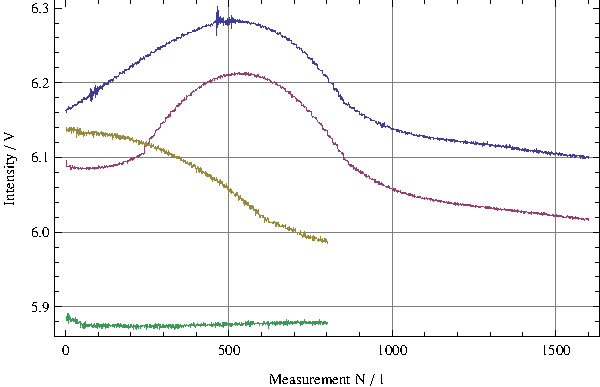
\includegraphics[width=0.45\linewidth]{img/drift.pdf}
\caption{
\small Measurements with active laser but without any coil currents. The top two (larger) measurements were taken over a time interval, that was about 4 times larger than the interval of a single regular measurement (i.e. the time needed to perform a full hysteresis loop), the lower two over a time of about two regular single measurements. } 
	\label{fig:waal}
\end{figure}


\subsection{Kerr Angle}
According to equation \Formel{eq:c} it is possible to calculate the Kerr angle from a set of contrast values. Preferably around the extinction angle as there is more change in contrast there. The measurements (when given the negative sign arbitrarily whenever the hysteresis curve goes from the bottom-left to the upper-right) allows for an easy fit of the functional relation derived previously for either the positive or the negative part. A combined fit of all data points results in a high variance, while the individual fits are very precise (cf. fig \ref{fig:kerrangle}).

The reason for this mismatch is not very obvious. A material defect seems unlikely, because it is a sudden effect around the extinction angle. Without further investigation, the best explanation includes interfering light reflexes at a horizontal angle on the photodiode and is rather far fetched. To get a better explanation, it would be necessary to go back to the setup and exclude possible reasons one by one.\footnote{It is most likely an error with the setup though. While J\"org and Anika only fitted the approximated formulas, they had the same problem we had. Their maximal values in the positive and negative part have the same asymmetry. \cite{jrganika}}

The individual fits give an averaged Kerr angle of $\Phi_K = (0.071\pm0.008)^\circ$ and an elliptic component of $I_1=(0.018\pm0.003)I_0$ of the light. This elliptic component is due to the imperfect alignment of the laser as well, so it can not be seen as a pure result of the Kerr effect.

A comparison to a literature value of $\Phi_\text{lit}=0.14 \degree$ (cf. \cite{stanford}) for longitudinal MOKE at $45\degree$ incidence, which matches the conditions of the experiment yields non compatible values, but comparable orders of magnitude.

\begin{figure} 
 \centering
         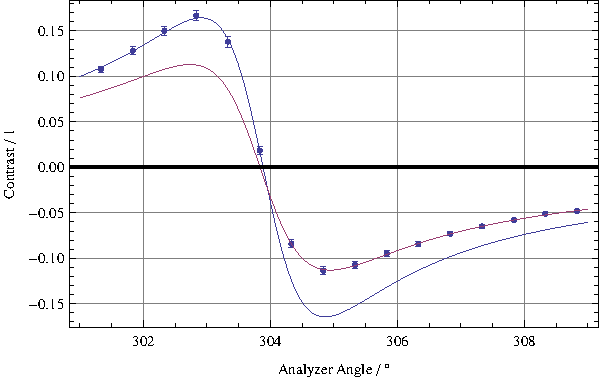
\includegraphics[width=0.45\linewidth]{img/kerr.pdf}
\caption{
\small Contrast over angle near the extinction of $304^\circ$. Fitted curves for positive and negative points result in: (positive points) $I_1 = -(0.017\pm0.005)I_0$, $\alpha_0=(303.89\pm 0.09)^\circ$, $\Phi_K=(0.080\pm0.015)^\circ$ and (negative points) $I_1 = -(0.019\pm0.003)I_0$, $\alpha_0=(303.84\pm 0.17)^\circ$, $\Phi_K=(0.062\pm0.005)^\circ$ in equation \ref{eq:c}. } 
	\label{fig:kerrangle}
\end{figure}


\subsection{Incidence Angle}
Apart from the angle of the analyser, the contrast also depends on the angle of the incident light relative to the normal of the surface. This dependence is plotted as measured in figure \ref{fig:inc}. For the s-polarized light, the non-linear component in the angle dependence is very small, almost non-existent, in agreement with the plots from \cite{paper}. The measurement of the p-polarized light could unfortunately not be evaluated. The values between $22.5^\circ$ and $35^\circ$ might be correct but the rest suffers an effect that has nothing to do with the phenomenon that we wanted to investigate. It is possible, that the light beam did not hit the sample properly or something similar. While we naturally tried to avoid this during the measurements, it still seems to be the best explanation in retrospect.
%TODO kein "we"?
\begin{figure} 
 \centering
\subfloat[][s-polarized]
{         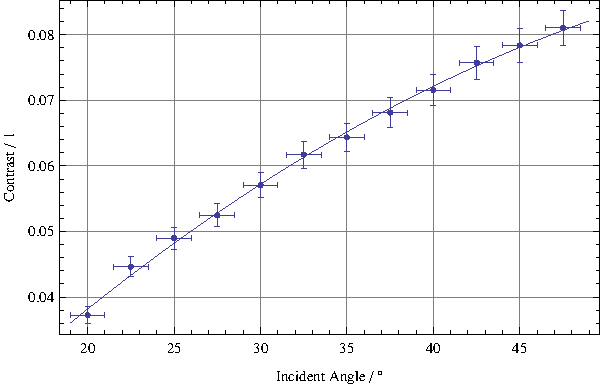
\includegraphics[width=0.45\linewidth]{img/incs.pdf}
       
}
\subfloat[][p-polarized]
         {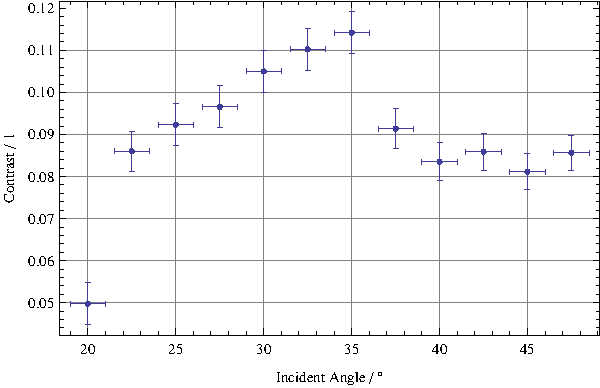
\includegraphics[width=0.45\linewidth]{img/incp.pdf}}

\caption{
\small Contrast over the angle between incident light and normal on the surface for s- and p-polarized light. The quadratic fit for the measurement of the s-polarized light has a non-linear component of $(2.0\pm2.8)\cdot 10^{-5}$. } 
	\label{fig:inc}
\end{figure}


\FloatBarrier


\subsection{Kerr Microscopy}



A thin film of iron-garnet is exposed to a magnetic field of tunable strength and analysed with a Kerr microscope. Due to the shape anisotropy caused by the geometry of the sample, we expect the magnetization of be within the plane. The domains, that can be seen are thus Bloch walls, where the magnetization is rotated around the normal vector of the plane. 

As the sample is considerably contaminated, there are only a few regions, in which the formation of magnetic domains is visible. Thus, only the qualitative properties of the domains are described and an estimate of the domain with by the comparison with a hair is not given.


\begin{figure} 
 \centering
\subfloat[][maze-structure]
{         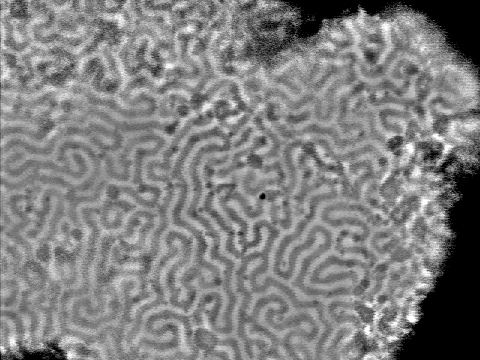
\includegraphics[width=0.3\textwidth]{img/andere1.pdf}} \hfill
\subfloat[][thin "walls"]
         {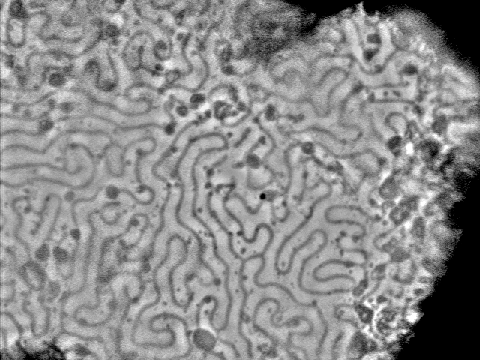
\includegraphics[width=0.3\textwidth]{img/andere2.pdf}} \hfill
\subfloat[][almost one-domain] 
         {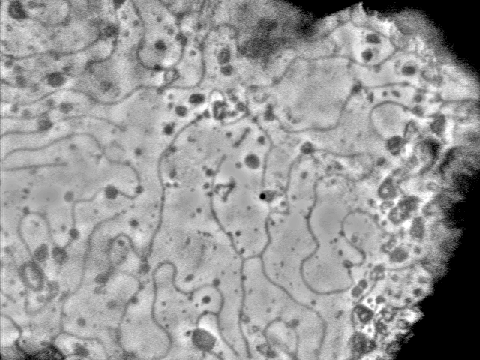
\includegraphics[width=0.3\textwidth]{img/andere3.pdf}} \hfill
\caption{ Changes of the domain structure during the increase of the external magnetic field. Transition from equal magnetization distribution \textbf{(a)} to enlarged favourable magnetization \textbf{(b)} to almost one-domain state \textbf{(c)}.
\small  } 
	\label{fig:domains}
\end{figure}

\begin{figure} 
 \centering
\subfloat[][before $H_{max}$]
{         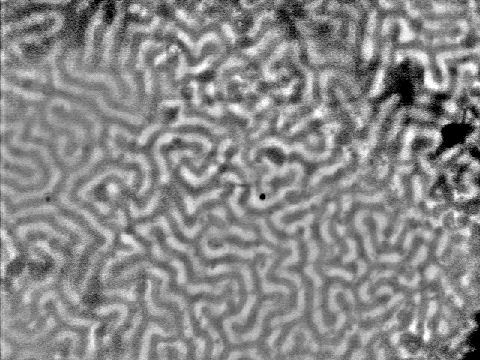
\includegraphics[width=0.45\textwidth]{img/domains2.pdf}} \hfill
\subfloat[][after $H_{max}$]
         {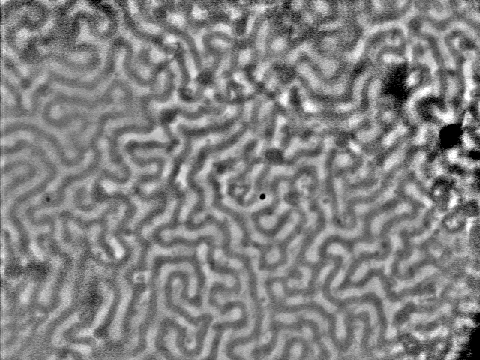
\includegraphics[width=0.45\textwidth]{img/reaufbau.pdf}} 
\caption{ \small \textbf{(a)} Domain state at increasing magnetic field. \textbf{(b)} Domain state at a decreasing magnetic field after magnetic saturation was reached. The two states reveal a similar structure, but the domains are not arranged exactly in the same way.
  } 
	\label{fig:reaufbau}
\end{figure}






The domain structure exhibits the typical maze-like structure. When the external magnetic field is increased, the domains of energetically favourable magnetization are enlarged and the domains of opposite magnetizations become thinner (cf. fig. \ref{fig:domains}). If the external field is increased even further, the walls collapse and larger regions emerge. At last, no domains with unfavourable magnetization remain and the sample is in a one-domain state. Decreasing the magnetic field again leads to a different pattern of the domain states. It is not possible to reproduce the same domain state again (cf. fig. \ref{fig:reaufbau}).

Another interesting feature is the switching of magnetization domains, which happens suddenly and not continuously while the increasing the magnetic field. This process is due to defects in the atomic lattice and is displayed in figure \ref{fig:defect}.
\begin{SCfigure}
    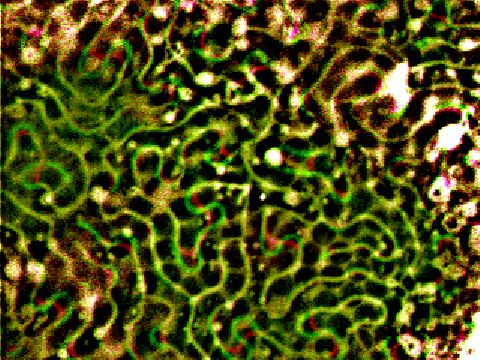
\includegraphics[width=0.48\textwidth]{img/kontrast.pdf}
  \caption{ \small Sudden changes in the magnetic domain structure at defects of the atomic lattice. The green lines display the structures, which are almost unchanged during a small increase of the magnetic field, while the red lines mark the sudden changes in the pattern. White spots display dirt on the sample. }
  	\label{fig:defect}
\end{SCfigure}

\clearpage

\section{Summary and Discussion}
The magneto-optical Kerr effect of a thin iron film was investigated in dependency of an external magnetic field, the direction of magnetization (hard and easy axes), and the polarization of the incoming laser beam as well as its incidence angle. 

The external magnetic field was generated by a toroid coil and calibrated against the current using a Hall probe. The magnetic anisotropy of the iron film was measured by making use of the Kerr rotation, that alters the polarization angle of a laser beam reflected on the sample's surface. A polarization filter was used to transform the change of the polarization angle into a change of the intensity of the laser beam, which was measured with a photodiode. Thus, the hysteresis loops along the easy axis [100] and a harder axes [110] could be recorded by placing the sample in two different positions with respect to the external field. The hysteresis loops showed the typical shapes for easy and hard axes and the difference of their enclosed areas was determined in order to calculate the anisotropy energy, that is necessary to change the magnetization of the sample.

The Kerr angle of the sample was determined by analysing the contrast of the intensities measured at the two saturation magnetizations points. Measuring the contrast as a function of the angle of the polarization analyser revealed the expected relation from which the Kerr angle could be determined to be $\SI{0.071(8)}{\degree}$. However, the curves of the measurements showed severe asymmetries with respect to the extinction angle, that could not be explained.

The dependency of the Kerr rotation on the incidence angle and polarization of the laser beam was successful for s-polarized light. It revealed an almost linear dependence between the contrast and the incidence angle, which was expected and is in good agreement with the measurements performed by  Zak et al. \cite{paper}. However, the same measurement for p-polarized light failed. Only for the first angles a linear behaviour was recorded. All further measurements revealed no reasonable data, most probably due to impurities of the sample.

At last the Kerr rotation was used in a Kerr microscope to analyse the domain structure of a thin iron-garnet film in a tunable magnetic field. The expected structures and behaviours of the magnetic domains and Bloch walls could fully be detected.

All in all the measurement can be considered successful, although it seemed like the electronic equipment was very sensitive to any disturbances and drift effects could be seen in the measurement data, which could not be suppressed by means of computation. It would be helpful to check all electronic devices in order to eliminate or reduce those effects. 
 \bibliographystyle{unsrt}
\bibliography{bib}

\end{document}
